\usepackage{listings}
\usepackage{graphicx}%! Author = phili
%! Date = 28/06/2021

\section{Integer Security}
\begin{itemize}
    \item Integer boundary concerns are often ignored
    \item Ariane 5 destroyed after integer overflow
    \item Results of integer overflow depend on the language and hardware
\end{itemize}
\textbf{Integer Promotion Example:}
\begin{lstlisting}
char c1, c2;
c1 = c1 + c2;
\end{lstlisting}

\subsection{Implicit Conversions}
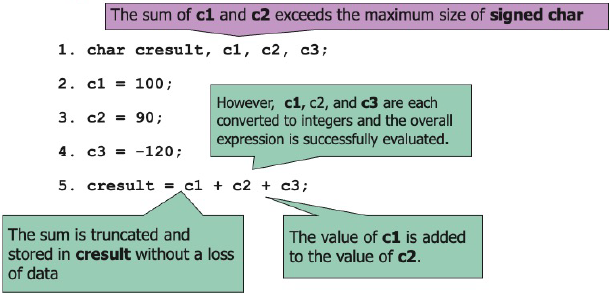
\includegraphics[width=\linewidth]{../img/implicit_conversions.png}

\subsection{Signed Integer Conversion}
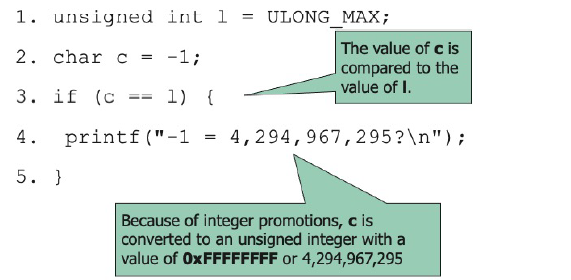
\includegraphics[width=\linewidth]{../img/signed_integer_conversion.png}

\subsection{Overflow Examples}
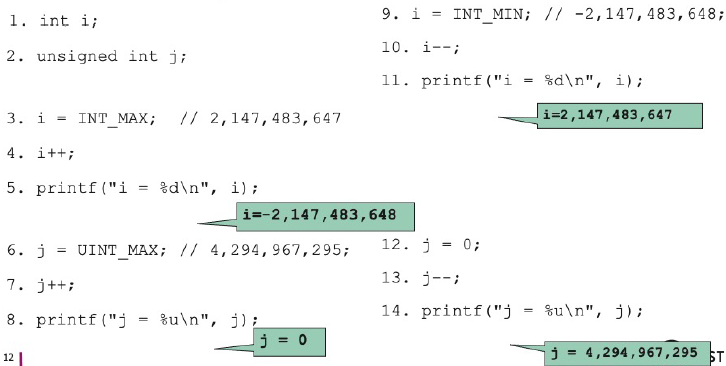
\includegraphics[width=\linewidth]{../img/overflow_examples.png}

\subsection{Truncation Error Example}
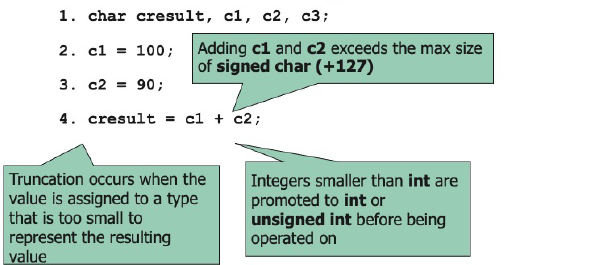
\includegraphics[width=\linewidth]{../img/truncation_error.png}
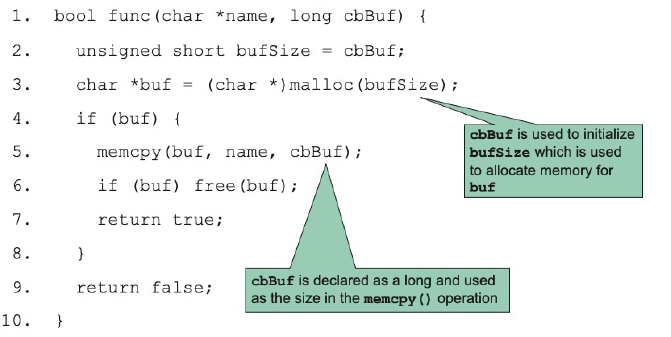
\includegraphics[width=\linewidth]{../img/truncation_error2.png}

\subsection{Sign Error Example}
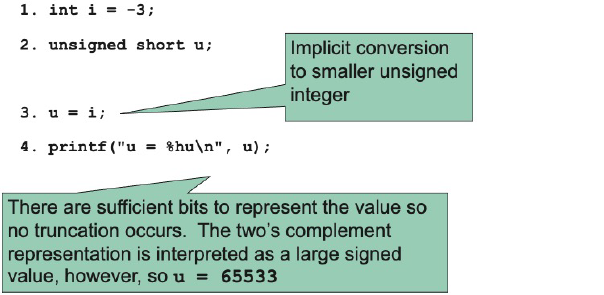
\includegraphics[width=\linewidth]{../img/sign_error.png}
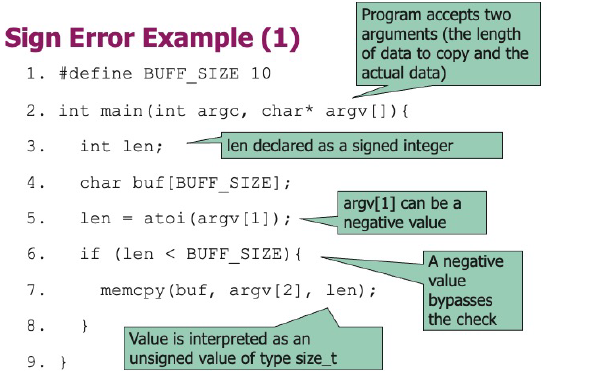
\includegraphics[width=\linewidth]{../img/sign_error2.png}

\subsection{Integer Division}
\begin{itemize}
    \item Minimum integer value divided by $-1$
    \item $-2'147'483'648 / -1 = -2'147'483'648$
\end{itemize}

\subsection{Negative Indices}
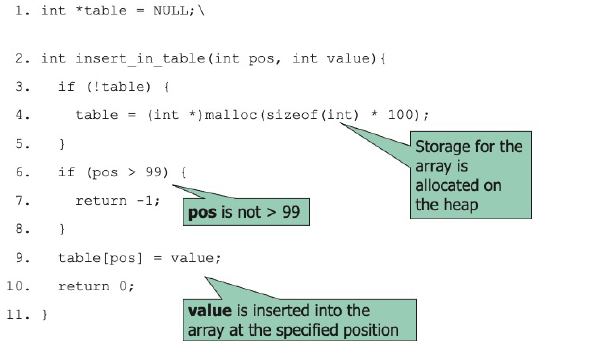
\includegraphics[width=\linewidth]{../img/negative_indices.png}

\subsection{Mitigation}
\textbf{Strong Typing}
\begin{itemize}
    \item Provide better types
    \item Using unsigned type to guarantee positive values
    \item Does not prevent overflow
\end{itemize}
\textbf{Abstract Data Type}
\begin{itemize}
    \item Create an abstract data type with private variables
    \item User can only changes values using public method calls
    \item Methods check valid range of input
\end{itemize}
\textbf{Safe Int Class}
\begin{itemize}
    \item C++ template class
    \item Tests the values of operands before performing an operation
\end{itemize}
\textbf{Testing}
\begin{itemize}
    \item Boundary checks
\end{itemize}
\textbf{Source Code Audit}
\begin{itemize}
    \item Source code should be audited or inspected
\end{itemize}